\section{Messages}
The protocol uses four main types of messages to communicate between 
the server and the clients. Those types are
\begin{description}
\item[Requests] A request is the basic way to communicate from the client 
  to the server and can be used either to query for some information or to 
  update the display. Some requests need a reply while other do not. 
  Requests needing a reply can be asyncrhonous or not.
\item[Replies] A reply is the basic way for the server to send back
  information to the client, and is usually used to send information about the server.
\item[Events] Events are generated by the server and sent to the client to notify it of 
  some event in the handled display. Event can be used for graphic events 
  (eg. when a window has been rendered) or for device events (eg. keyboard or mouse event).
\item[Errors] Errors can be generated from the client as well as the server
  for many different reasons. One of the main reason for errors generated 
  from the server side is for access to non available resources.
\end{description}
An overview of how these messages are sent is shown in figure~\ref{fig:xcore-overview}.
\begin{figure}[tb]
  \begin{center}
    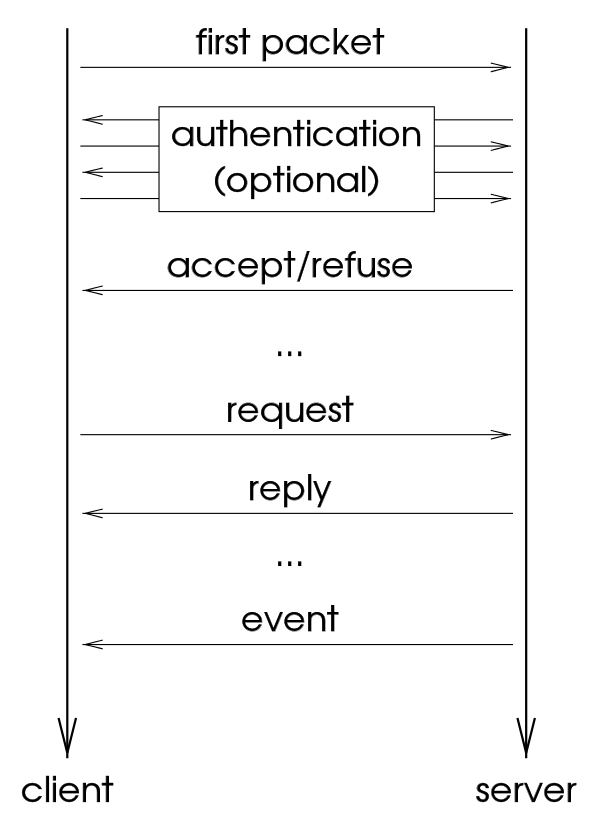
\includegraphics[height=8cm,width=6cm]{imgs/xcore-overview.png}
    \caption{\label{fig:xcore-overview}Overview of the X protocol \protect\footnotemark}
  \end{center}
\end{figure}